\documentclass[aspectratio=169]{beamer}

\usepackage[utf8]{inputenc}
\usepackage[T1]{fontenc}
\usepackage[brazil]{babel}
\usepackage{graphicx}
\usepackage{booktabs}
\usepackage{array}
\usepackage{colortbl}

\usetheme{Singapore}

\title[PHVD-APS -- Projeto de Pesquisa]{Planejamento de Visitas Domiciliares na APS\\}
\subtitle{INF99003 -- Projeto 2 -- Grupo D}
\author{Fabio, Tobias e V\'itor}
\date{Semana 2 -- 25/09/2026}

\setbeamertemplate{navigation symbols}{}
\setbeamercovered{transparent}
\setbeamertemplate{footline}[frame number]

% ── colour helpers ──────────────────────────────────────────────────────────
\definecolor{myblue}{RGB}{30,80,160}
\definecolor{myorange}{RGB}{210,100,20}
\definecolor{mygreen}{RGB}{30,130,60}
\definecolor{mygray}{RGB}{90,90,90}

\begin{document}

% ============================================================
\begin{frame}
  \titlepage
\end{frame}

% ============================================================
\section{Problema}

\begin{frame}{O problema}
  \begin{columns}[T]
    \column{0.48\textwidth}
      \textbf{Contexto}
      \begin{itemize}
        \item Equipes ESF realizam \textbf{visitas domiciliares peri\'odicas}
        \item Planejamento hoje: \textbf{manual} ou sem suporte computacional
      \end{itemize}
      \vspace{0.4em}
      \textbf{Consequ\^encias}
      \begin{itemize}
        \item Ac\'umulo de \textbf{pend\^encias}
        \item Rotas \textbf{ineficientes}
        \item Carga \textbf{desigual} entre equipes
      \end{itemize}
    \column{0.48\textwidth}
      \textbf{4 decis\~oes interdependentes:}
      \vspace{0.3em}
      \begin{enumerate}
        \item \textbf{Selecionar} quais visitas realizar
        \item \textbf{Escolher} o dia de atendimento
        \item \textbf{Atribuir} a uma equipe
        \item \textbf{Ordenar} a sequ\^encia de casas
      \end{enumerate}
      \vspace{0.4em}
  \end{columns}
\end{frame}

% ============================================================
\begin{frame}{Pergunta e hip\'otese}
  \begin{block}{Pergunta de pesquisa}
    Em inst\^ancias representativas de visitas domiciliares e falhas de
    atendimento, quanto uma \textbf{heur\'istica de janela m\'ovel de N dias}
    melhora pend\^encias, atraso acumulado e deslocamento em rela\c{c}\~ao a
    regras simples de planejamento?
  \end{block}
  \vspace{0.5em}
  \begin{alertblock}{Hip\'otese}
    Sele\c{c}\~ao por \textbf{urg\^encia + prazos futuros} + inser\c{c}\~ao de
    menor custo + \textbf{2-opt} reduz atraso acumulado sem elevar
    excessivamente deslocamento ou tempo computacional.
  \end{alertblock}
\end{frame}

% ============================================================
\section{Modelo}

\begin{frame}{Entidades e dados de entrada}
  \centering
  \small
  \begin{tabular}{@{}lll@{}}
    \toprule
    \textbf{Entidade} & \textbf{Campos-chave} & \textbf{Papel no modelo} \\
    \midrule
    Posto de sa\'ude   & coordenadas            & Origem/destino de todas as rotas \\
    Equipe             & jornada $H_{k,t}$, disponib. & Capacidade diária \\
    Paciente           & coordenadas, dura\c{c}\~ao $s_i$ & N\'o do grafo \\
    Condi\c{c}\~ao     & intervalo máximo, prioridade & Define prazo da visita \\
    Resultado          & conclu\'ido / n\~ao realizado & Atualiza hist\'orico \\
    Janela             & $N$ dias \'uteis, anteciap.\,$A$ & Horizonte m\'ovel \\
    \bottomrule
  \end{tabular}
\end{frame}

% ============================================================
\begin{frame}{Regras temporais}
  \begin{columns}[T]
    \column{0.50\textwidth}
      \textbf{Data-limite} por condi\c{c}\~ao:
      \[
        d_{\text{lim}} = \text{\'ult.\ visita} + \text{intervalo}
      \]
      \textbf{Atraso} (dias):
      \[
        \text{atraso} = \max(0,\; \text{hoje} - d_{\text{lim}})
      \]
      \textbf{Antecipa\c{c}\~ao}: visita pode ser agendada at\'e $A$ dias
      \emph{antes} do prazo.

    \column{0.46\textwidth}
      \textbf{Estados de uma visita:}
      \begin{itemize}
        \item \textcolor{red!70!black}{\textbf{Vencida}} — prazo anterior ao dia
        \item \textcolor{orange!80!black}{\textbf{Vence hoje}}
        \item \textcolor{myblue}{\textbf{Futura}} — dentro da janela
      \end{itemize}
      \vspace{0.4em}
      Somente \textbf{conclus\~ao} atualiza a data real.\\
      Visita n\~ao realizada volta \`a fila com prazo original.
  \end{columns}
\end{frame}

% ============================================================
\section{Artefato}

\begin{frame}{Pipeline de execu\c{c}\~ao}
  \centering
  \vspace{-0.2cm}
  \makebox[\textwidth][c]{%
    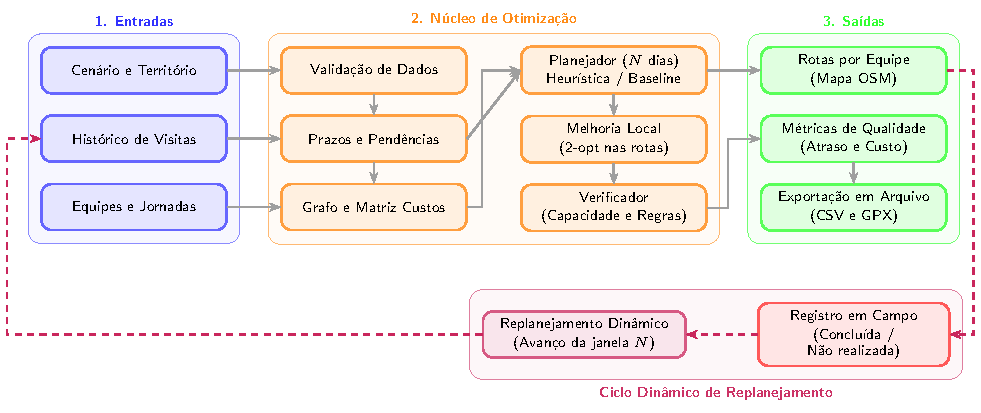
\includegraphics[width=1.08\textwidth,height=0.82\textheight,keepaspectratio]{figs/pipeline.pdf}%
  }
\end{frame}

% ============================================================
\begin{frame}{Interface m\'inima}
  \centering
  \small
  \begin{tabular}{@{}lll@{}}
    \toprule
    \textbf{Tela} & \textbf{A\c{c}\~oes} & \textbf{Retorno} \\
    \midrule
    Cadastros        & Criar/editar posto, pacientes, equipes   & Valida\c{c}\~ao e erros \\
    Mapa de entrada  & Marcar posto/casas; desenhar polgonos    & Coordenadas persistidas \\
    Mapa de sa\'ida  & Selecionar dia; ver todas as equipes     & Rotas coloridas + legenda \\
    Exporta\c{c}\~ao & Baixar \textbf{CSV} e \textbf{GPX}      & Arquivo por equipe/dia \\
    Execu\c{c}\~ao   & Marcar resultado; encerrar dia           & Nova vers\~ao do plano \\
    \bottomrule
  \end{tabular}
  \vspace{0.4em}

\end{frame}

% ============================================================
\section{M\'etodos}

\begin{frame}{M\'etodos implementados e comparados}
  \begin{enumerate}
    \item \textbf{Baseline urg\^encia:} ordenar por vencimento; inserir na equipe de menor custo adicional
    \item \textbf{Baseline geogr\'afico:} vizinho vi\'avel mais pr\'oximo (nearest-neighbor)
    \item \textbf{Heur\'istica principal:} pontuar por atraso + peso cl\'inico + proximidade do prazo + custo incremental; permite antecipar dentro de $A$; pend\^encias t\^em prioridade sobre futuras
    \item \textbf{Melhoria local (2-opt):} reduzir deslocamento dentro de cada rota sem mudar dias
    \item \textbf{Refer\^encia exata} (\emph{opcional}): enumera\c{c}\~ao em inst\^ancias pequenas
  \end{enumerate}
  \vspace{0.3em}
  {\small Todos recebem o mesmo estado inicial, calend\'ario e sequ\^encia de eventos reais.}
\end{frame}

% ============================================================
\section{Experimentos}

\begin{frame}{Cen\'arios e m\'etricas}
  \begin{columns}[T]
    \column{0.48\textwidth}
      \textbf{Cen\'arios}
      \begin{itemize}
        \item Capacidade: folgada / equilibrada / insuficiente
        \item Distribui\c{c}\~ao: pr\'oximos / espalhados
        \item Pend\^encias: poucas / muitas, atraso variado
        \item Falhas: isoladas / sucessivas
        \item Casos-limite: 0 pacientes, fora do pol\'igono, etc.
      \end{itemize}
    \column{0.48\textwidth}
      \textbf{M\'etricas}
      \begin{itemize}
        \item Fra\c{c}\~ao de pend\^encias conclu\'idas
        \item Dias de \textbf{atraso acumulado}
        \item Deslocamento efetivo e planejado
        \item Utiliza\c{c}\~ao e desequil\'ibrio de jornada
        \item Tempo de gera\c{c}\~ao / replanejamento
        \item Mem\'oria m\'axima
      \end{itemize}
      \vspace{0.2em}
      {\small Plano previsto $\neq$ resultado simulado.}
  \end{columns}
\end{frame}

% ============================================================
\section{Pr\'oximos Passos}

\begin{frame}{Pr\'oximas Semanas -- Pr\'oximos Passos}
  \small
  \begin{columns}[T]
    \column{0.48\textwidth}
      \textbf{\textcolor{myblue}{1. Implementa\c{c}\~ao}} \hfill {\footnotesize\textcolor{mygray}{(Semana 3)}}
      \begin{itemize}
        \item \textbf{N\'ucleo}: gerador sint\'etico, matriz Haversine e regras temporais
        \item \textbf{M\'etodos}: baselines, heur\'istica com antecipa\c{c}\~ao e 2-opt
        \item \textbf{Interface}: mapa OSM e exporta\c{c}\~ao \textbf{CSV e GPX}
      \end{itemize}

      \vspace{0.7em}
      \textbf{\textcolor{myorange}{2. Experimenta\c{c}\~ao}} \hfill {\footnotesize\textcolor{mygray}{(Semana 4)}}
      \begin{itemize}
        \item Execu\c{c}\~ao em lote com sementes fixadas
        \item Varia\c{c}\~ao de capacidade, dist\^ancias e falhas no horizonte m\'ovel
      \end{itemize}

    \column{0.48\textwidth}
      \textbf{\textcolor{mygreen}{3. An\'alise de Resultados}} \hfill {\footnotesize\textcolor{mygray}{(Semana 4)}}
      \begin{itemize}
        \item Heur\'istica vs.\ baselines (atraso acumulado vs.\ deslocamento)
        \item Fronteira de Pareto e sensibilidade
        \item Valida\c{c}\~ao emp\'irica da complexidade
      \end{itemize}

      \vspace{0.7em}
      \textbf{\textcolor{purple!80!black}{4. Reda\c{c}\~ao do Artigo}} \hfill {\footnotesize\textcolor{mygray}{(Semana 4)}}
      \begin{itemize}
        \item Gr\'aficos, tabelas e interpreta\c{c}\~ao
        \item Discuss\~ao cr\'itica de amea\c{c}as \`a validade
        \item Escrita e revis\~ao do relat\'orio final
      \end{itemize}
  \end{columns}
\end{frame}

% ============================================================
\begin{frame}{Refer\^encias}
  \begin{columns}[T]
    \column{0.48\textwidth}
    \begin{itemize}
      \item Barros et al.\ (2022)
      \item Matta \& Morosini (Fiocruz)
      \item Faria (2020)
      \item Rodrigues et al.\ (2014)
    \end{itemize}
    \column{0.48\textwidth}
    \begin{itemize}
      \item CONASS (2021)
      \item Pinto \& Rocha (2024)
      \item Bender et al.\ (2021)
      \item \textbf{Randriamihaja et al.\ (2024)}
    \end{itemize}
  \end{columns}
\end{frame}

% ============================================================
\begin{frame}{}
  \centering
  \vspace{1cm}
  {\Huge Obrigado!}\\[1em]
  {\large D\'uvidas e discuss\~ao}
\end{frame}

\end{document}
